%libro Paul R. Gray, Paul J. Hurst, Stephen H. Lewis, Robert G. Meyer - Analysis and Design of Analog Integrated Circuits (2001, Wiley) capitulo feedback revista todoelectronica fasciculo segundo.
\paragraph{}
La realimentación es un concepto ligado a la amplificación.
La realimentación, en los amplificadores, consiste en tomar una muestra de tensión o de corriente a la salida y reenviarla a la entrada a través de una red apropiada.
Gracias a la realimentación se consigue estabilizar la ganancia, la resistencia de entrada, la resistencia de salida y el ancho de banda, aunque el fin más importante es la estabilización de la ganancia\footnote{\textit{Revista Todoelectrónica}. (n.d.). Fascículo segundo.}.
\paragraph{}
En la figura \ref{fig:fb} se muestra el esquema general de un sistema realimentado, donde $A$ se corresponde con la ganancia en lazo abierto del amplificador, y $f$ la red de realimentaci\'on correspondiente. Dependiendo de la naturaleza del amplificador y del tipo de realimentación, la ganancia en lazo abierto puede ser de tensión, corriente, transimpedancia o transconductancia.
\begin{figure}[h]
    \centering
    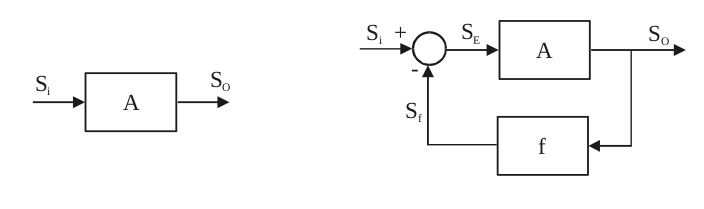
\includegraphics[scale=1, width=.7\textwidth]{fb}
    \caption{a) Amplificador sin realimentaci\'on, b) Sistema realimentado} 
    \label{fig:fb}
\end{figure}
\paragraph{}
En la figura \ref{fig:fb} se calculan las ganancias propias de cada sistema. La nomenclatura $S_n$ se refiere a una señal que bien puede ser de corriente o tensión.
Por un lado, la ganancia en lazo abierto del amplificador se calcula como:
$$A = \frac{S_o}{S_i} $$
Por otro lado, se calcula la ganancia en lazo cerrado $A_f$:
\[
\begin{array}{rccl} 
      \begin{array}{l}
	 \begin{cases}
	    S_f = S_o \cdot f \\
	    S_E = S_i - S_f \\
	    S_o = S_E \cdot A
	 \end{cases}
      \end{array}
      &
      \begin{array}{l}
	  =>
      \end{array}
      &
      \begin{array}{l}
	 \frac{S_o}{A} = S_i - S_o \cdot f \\
	 S_i = S_o \cdot \left(\frac{1}{A} + f \right) = S_o \cdot \frac{1}{A} \cdot (1 + f \cdot A) \\
	 A_f = \frac{S_o}{S_i}
      \end{array}
      &
      \begin{array}{l}
	 A_f = \frac{S_o}{S_i} = \frac{A}{(1 + f \cdot A)} 
      \end{array}
\end{array}
\]
\paragraph{}
Se señalan las ecuaciones que ser\'an de utilidad:
\begin{align}
   \label{eq:feedback}
   A_f &= \frac{S_o}{S_i} = \frac{A}{(1 + f \cdot A)} \\
   \label{eq:A}
   A &= \frac{S_o}{S_E} \\
   \label{eq:Al}
   A_l &= A \cdot f
\end{align}
\paragraph{}
Es útil definir el par\'ametro ganancia en lazo abierto, $A_l = A \cdot f$, para poder analizar el comportamiento del sistema en lazo cerrado cuando $A_l$ var\'ia. Esto se conoce como el criterio de Barkhausen, el cual se expone considerando el criterio de signos de la ecuaci\'on \ref{eq:feedback}:
\begin{itemize}
   \item \textbf{Si $\mathbf {A_l >> 1}$:} en este caso se obtiene una ganancia total del sistema $A_f = \frac{1}{f}$. Esta realimentación se conoce como negativa.
   \item \textbf{Si $\mathbf{A_l << 0}$:} en este caso se tiene que $S_E = S_i + S_f$, es decir, las señales se encuentran en fase y se suman en lugar de restarse. Esta suma es amplificada una y otra vez dando lugar a un sistema inestable. Esta realimentación se conoce como positiva.
   \item \textbf{Si $\mathbf{A_l = -1}$:} en este caso el sistema se encuentra en la frontera entre la estabilidad y la inestabilidad. Por lo que idealmente, el sistema responder\'a a la funci\'on impulso o delta de Dirac con una oscilaci\'on continuada. Este caso es conocido como el criterio de Barkhausen y se trata de la condici\'on necesaria para encontrar oscilaciones\footnote{Gray, P. R., Hurst, P. J., Lewis, S. H., \& Meyer, R. G. (2001). \textit{Analysis and Design of Analog Integrated Circuits}. Wiley. Capítulo 8: Feedback.}.
\end{itemize}
\paragraph{}
Por último, se han de mencionar los diferentes tipos de realimentación que se dan en los amplificadores prácticos. Como se ha mencionado anteriormente, las señales de trabajo pueden ser de tensión, corriente o incluso una combinación de ambas. De esta forma, se pueden clasificar los diferentes tipos de realimentación en función de la señal de trabajo tanto a la entrada como a la salida. Alugnos de estos tipos se exponen en las figuras \ref{fig:sp} y \ref{fig:pp}\footnote{González Díaz, G. (n.d.). \textit{Apuntes de electrónica analógica}. Cap\'itulo 7: Realimentaci\'on negativa}.
\begin{figure}[H]
    \centering
    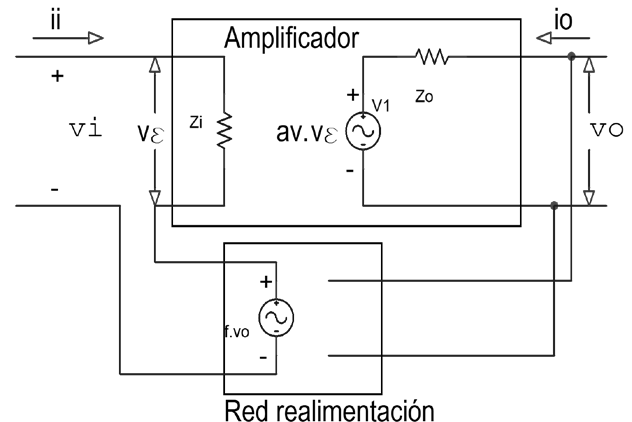
\includegraphics[scale=1, width=.4\textwidth]{sp-tension}
    \caption{Amplificador de tensión con realimentaci\'on serie paralelo ideal.} 
    \label{fig:sp}
\end{figure}

\begin{figure}[H]
    \centering
    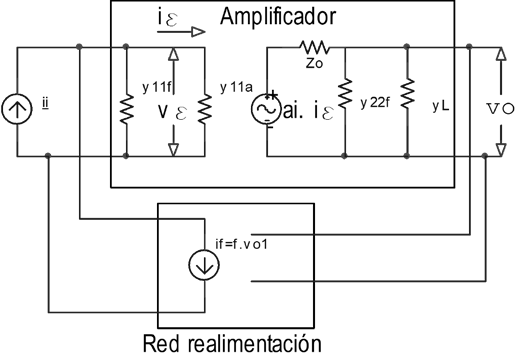
\includegraphics[scale=1, width=.4\textwidth]{pp-transres-real}
    \caption{Amplificador de transresistencia con realimentación paralelo paralelo real.} 
    \label{fig:pp}
\end{figure}
